\documentclass[a4paper,11pt]{article}
\usepackage{pdflscape}
\usepackage[utf8]{inputenc}
\usepackage[T1]{fontenc}
%\usepackage{fourier} % math & rm
%\usepackage{amsthm,amsfonts,amsmath,amssymb,textcomp}
\usepackage{pst-all,pstricks-add,pst-eucl}
\everymath{\displaystyle}
\usepackage{fp,ifthen}
%\usepackage{color}
%\usepackage{graphicx}
\usepackage{setspace}
\usepackage{array}
\usepackage{tabularx}
\usepackage{supertabular}
\usepackage{hhline}
\usepackage{variations}
\usepackage{enumerate}
\usepackage{pifont}
\usepackage{framed}
\usepackage[fleqn]{amsmath}
\usepackage{amssymb}
\usepackage[framed]{ntheorem}
\usepackage{multicol}
\usepackage{kpfonts}
\usepackage{manfnt}

%\usepackage[hmargin=2.5cm, vmargin=2.5cm]{geometry}
\usepackage{vmargin}          % Pour fixer les marges du document
\setmarginsrb
{1.5cm} 	%marge gauche
{0.5cm} 	  %marge en haut
{1.5cm}     %marge droite
{0.5cm}   %marge en bas
{1cm} 	%hauteur de l'entête
{0.5cm}   %distance entre l'entête et le texte
{1cm} 	  %hauteur du pied de page
{0.5cm}     %distance entre le texte et le pied de page

\newcommand{\R}{\mathbb{R}}
\newcommand{\N}{\mathbb{N}}
%\newcommand{\D}{\mathbb{D}}
\newcommand{\Z}{\mathbb{Z}}
\newcommand{\Q}{\mathbb{Q}}
\newcommand{\C}{\mathbb{C}}
\newcommand{\e}{\text{e}}
\newcommand{\dx}{\text{d}x}
\newcommand{\vect}[1]{\mathchoice%
  {\overrightarrow{\displaystyle\mathstrut#1\,\,}}%
  {\overrightarrow{\textstyle\mathstrut#1\,\,}}%
  {\overrightarrow{\scriptstyle\mathstrut#1\,\,}}%
  {\overrightarrow{\scriptscriptstyle\mathstrut#1\,\,}}}
\newcommand\arraybslash{\let\\\@arraycr}
\renewcommand{\theenumi}{\textbf{\arabic{enumi}}}
\renewcommand{\labelenumi}{\textbf{\theenumi.}}
\renewcommand{\theenumii}{\textbf{\alph{enumii}}}
\renewcommand{\labelenumii}{\textbf{\theenumii.}}
\renewcommand{\and}{\wedge}

\theoremstyle{break}
\theorembodyfont{\upshape}
\newframedtheorem{theorem}{Théorème}
\newframedtheorem{Prop}{Proposition}
\newframedtheorem{Def}{Définition}

\newtheorem{Term}{Terminologie}
\newtheorem{Rq}{Remarque}
\newtheorem{exemple}{Exemple}
%\newtheorem{exo}{Exercice}

%\theorembodyfont{\small \sffamily}
%\newtheorem{sol}{solution}

\newenvironment{sol}% 
{\def\FrameCommand{\hspace{0.5cm} {\color{black} \vrule width 1pt} \hspace{-0.7cm}}%
  \framed {\advance\hsize-\width}
  \noindent \small \sffamily  %\underline{Solution :}%\\
}%
{\endframed}

\newrgbcolor{vert}{0 0.4 0}
\newrgbcolor{bistre}{1 .50 .30}
\setlength\tabcolsep{1mm}
\renewcommand\arraystretch{1.3}

\everymath{\displaystyle}
\hyphenpenalty 10000 %supprime toutes les césures
%\setcounter{secnumdepth}{0}
%\newcounter{saveenum}

\usepackage[frenchb]{babel}
\usepackage{fancyhdr,lastpage}
\usepackage{fancybox}

%\headheight 15.0 pt
\fancyhead[L]{}
\fancyhead[C]{Second degré}
\fancyhead[R]{}
\fancyfoot[L]{{\scriptsize\textsl{Thomas Gire Cité scolaire de Lorgues}}}
%\fancyfoot[C]{\scriptsize\thepage}
%\fancyfoot[C]{\scriptsize\thepage/\pageref{LastPage}}

\title{}
\author{}
\date{}

%\pagestyle{empty}
\pagestyle{fancy}
\usepackage[np]{numprint}

\renewcommand\arraystretch{1.8}

\newcounter{numero}
\newcommand{\exo}{
  \addtocounter{numero}{1}%
  \textbf{\underline{Exercice \arabic{numero}:}}\quad}

\frenchbsetup{StandardEnumerateEnv=true}
\usepackage{etex}
\usepackage{tikz,tkz-tab}
\usepackage{graphicx}
\graphicspath{ {../images/} }

\begin{document}
  \setlength{\unitlength}{1mm}
  \setlength\parindent{0mm}
  
  
  %\exo
  ~
  \medskip
  
  \section{Rappels de la classe de seconde.}
  
  \subsection{Variations de fonctions.}
  
  \begin{Def}
    Une fonction est \textbf{croissante} (respectivement \textbf{décroissante}) sur un
    intervalle si les images de nombres dans cet intervalle sont rangées dans le même
    ordre (respectivement l'ordre inverse) que ces nombres.
  \end{Def}
  
  \begin{exemple}
    La fonction carré $\R \to \R, x \mapsto x^2$ est décroissante sur $]-\infty;0]$. 
    Par exemple, $(-2)^2=4>1=(-1)^2$. Pour exhiber les variations d'une fonction, 
    on construit souvent un tableau.
    
    \begin{tikzpicture}
      \tkzTabInit{$x$/1,$x^2$/2}{$-\infty$, $0$}
      
      \tkzTabVar{+/$+\infty$,-/$0$}
    \end{tikzpicture}
  \end{exemple}
  
  
  
  \begin{Def}
    Le \textbf{minimum} (respectivement le \textbf{maximum}) d’une fonction
    sur un intervalle est la plus petite (respectivement la plus grande) 
    valeur atteinte par cette fonction sur cet intervalle.
    %Autrement dit, $m$ est le \textbf{minimum} (respectivement le \textbf{maximum}) de 
    %la fonction $f:E \to \R$ s'il existe $x_0$ dans $E$ tel que pour tout x 
    %dans $E$, ${m \leq f(x)}$ (respectivement $m \geq f(x)$).
    
    On appelle \textbf{extremum}, un minimum ou un maximum.
  \end{Def}
  
  \begin{exemple}
    D'après le tableau de variations précédent, 0 est le minimum de la fonction
    $f:]-\infty ; 0] \to \R, x \mapsto x^2$. Il est atteint pour $x=0$ et $f(x)$
    ne possède pas de maximum.
  \end{exemple}
  
  \subsection{Trinôme du second degré.}
  
  \begin{Def}
   On dit qu'une fonction $f$ est un trinôme du second degré si elle peut se mettre
   sous la forme $f(x)=ax^2+bx+c$ où $a,b,c$ sont trois nombres rééls avec $a$ non nul.
  \end{Def}
  
  \begin{exemple}
    \begin{itemize}
     \item La fonction $g(x)=2x^2+3x+1$ est un trinôme du second degré.
     \item La fonction $h(x)=3(x-1)^2+1=3(x^2-2x+1)+1=3x^2-6x+4$ est un trinôme 
     du second degré.
     \item La fonction $i(x)=4(x-1)(x+2)=4(x^2-x+2x-2)=4x^2+4x-8$ est un trinôme
     du second degré.
     \item La fonction affine $i(x)=5x+3$ n'est pas un trinôme du second degré.
     \item Le polynôme $j(x)=x^3+4x^2+1$ n'est pas un trinôme du second degré.
 \end{itemize} 
 \end{exemple}

  
  \newpage
  
  \subsection{Variations d'un trinôme du second degré}
  
  \begin{theorem}

    Un polynôme de degré 2, $f(x)=ax^2+bx+c$ admet pour variations:
    \begin{itemize}
      \item Si $a>0$
      \[
      \begin{tikzpicture}
	\tkzTabInit{$x$ /1,$f(x)$/2}{$-\infty$, $\alpha$, $+\infty$}
	
	\tkzTabVar{+/$+\infty$,-/$\beta$,+/$+\infty$}
      \end{tikzpicture}
      \] 
      
      \item Si $a<0$
      \[
      \begin{tikzpicture}
	\tkzTabInit{$x$/1,$f(x)$/2}{$-\infty$, $\alpha$, $+\infty$}
	
	\tkzTabVar{-/$-\infty$,+/$\beta$,-/$-\infty$}
      \end{tikzpicture}
      \]
    \end{itemize}
    
    On peut calculer les coordonnées $(\alpha,\beta)$ du sommet $S$ de la parabole grâce aux formules 
    $$\alpha=-\frac{b}{2a} \hspace{1cm} \beta=f(\alpha)$$
    
    \end{theorem}
    
      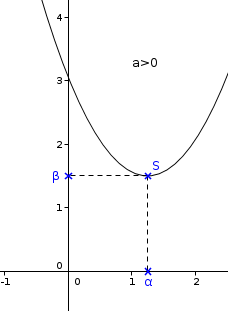
\includegraphics{variationsapos}\hspace{1cm}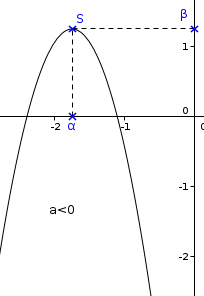
\includegraphics{variationsaneg}
    

     
     \section{Intersection d'une parabole avec l'axe des abscisses.}
    
    \begin{Prop}[Positions de paraboles]
    Il n'y a que deux possibilités pour une parabole $\mathcal{P}:y=a(x-\alpha)^2+\beta$ 
    de couper l'axe des abscisses en deux points:
   \begin{itemize}
    \item Soit elle admet un minimum strictement négatif (cas $a>0$ et $\beta <0$).
    \item Soit elle admet un maximum strictement positif.(cas $a<0$ $et$ $\beta >0$)
   \end{itemize}
   
   La parabole est tangente à l'axe des abscisses si et seulement si son extremum est 
   nul ($\beta=0$).

  \end{Prop}
  
  %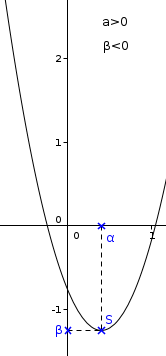
\includegraphics[width=4cm]{aposbetaneg}\hspace{0.3cm}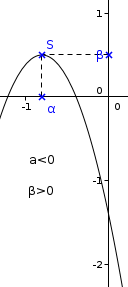
\includegraphics[width=4cm]{anegbetapos}
  
  \subsection{Racines d'un trinôme.}
  
  \begin{Def}
    Soit $f(x)=ax^2+bx+c$ un trinôme du second degré et son graphe $\mathcal{P}:y=f(x)$.
    \begin{itemize}
     \item 
    Si $\mathcal{P}$ coupe l'axe des abscisses en deux points 
    $A_1(x_1,0)$ et $A_2(x_2,0)$,
    on dit que \mbox{ $x_1$ et $x_2$ sont les} deux \textbf{racines} 
    du trinôme du second degré $f(x)$.
    
    \item
    Si une parabole $\mathcal{P}:y=ax^2+bx+c$ coupe l'axe des abscisses en un seul 
    point $A_0(x_0,0)$, on dit que $x_0$ est la \textbf{racine double} du trinôme du second 
    degré $f(x)$.
    
    
    \end{itemize}

    
    Autrement dit, $x$ est une racine de $f(x)$ si et seulement si $f(x)=0$.
  \end{Def}
  
  \begin{exemple}
    Soit $f(x)=3(x+1)(x-2)=3x^2-3x-6$. $-1$ et $2$ sont les deux racines de $f(x)$.\newline
    En effet, $f(-1)=3(-1+1)(-1-2)=3\times0 \times -3=0$ et $f(2)=3(2+1)(2-2)=3 \times 3 \times 0=0$.
    
    Soit $g(x)=2(x-3)^2=2(x^2-6x+9)=2x^2-12x+18$. $3$ est racine double. 
    En effet, $g(3)=2\times 0^2=0$ et pour tout $x \neq 3$,$x-3\neq0$ par suite 
    $(x-3)^2 \neq 0$ et en définitive $g(x)=2(x-3)^2 \neq 0$. 
  \end{exemple}
  
  \begin{Prop}[Reformulation de la proposition de la position d'une parabole]
    \begin{itemize}
     \item Un trinôme du second degré admet deux racines si et seulement si $a$ et $\beta$
   sont de signes contraires ou encore si et seulement si $a\beta<0$.
     \item Un trinôme du second degré admet une racine double si et seulement si
     $\beta=0$.
    \end{itemize}
  \end{Prop}
  
  \subsection{Calcul des racines et factorisation.}
  
  \begin{Def}[Discriminant]
    Soit $f(x)$ un trinôme du second degré dont la forme développée réduite
    est $f(x)=ax^2+bx+c$. On appelle \textbf{discriminant} de ce trinôme
    le nombre $\Delta=b^2-4ac$.
    
    On admet que $\beta=-\frac{\Delta}{4a}$.
  \end{Def}
  
  \begin{exemple}
    \begin{itemize}
     \item Soit $h(x)=x^2-4x+3$, $\Delta=4^2-4 \times 3=4=2^2>0$.
     \item Soit $i(x)=2x^2-4x+2$, $\Delta=4^2-4 \times 2 \times 2=0$.
     \item Soit $j(x)=-3x^2+12x-15$, $\Delta=12^2-4(-3)(-15)=144-180<0$
    \end{itemize}
   \end{exemple}
  
  \begin{theorem}[Central]
    Soit $f(x)=ax^2+bx+c$ un trinôme du second degré sous forme développée réduite.
    \begin{itemize}
     \item  $f(x)$ admet deux racines $x_1$,$x_2$ si et seulement si 
     son discriminant est strictement positif.
     
     Dans ce cas, on a:
     $$x_1=\frac{-b-\sqrt{\Delta}}{2a} \hspace{2cm} x_2=\frac{-b+\sqrt{\Delta}}{2a}$$
     
     Et le trinôme peut se factoriser en $f(x)=a(x-x_1)(x-x_2)$.
     
     \item $f(x)$ admet une racine double $x_0$ si et seulement si
     son discriminant est nul.
     
     Dans ce cas, on a :
     $$x_0=-\frac{b}{2a}(=\alpha)$$
     
     Et le trinôme peut se factoriser en $f(x)=a(x-x_0)^2$.
     
     \item $f(x)$ ne possède pas de racine si et seulement si son discriminant
     est strictement négatif.
     
     Dans ce cas $f(x)$ ne peut pas se factoriser en un produit de termes de degré 1.
    \end{itemize}    
  \end{theorem}
  
  \begin{exemple}
    On reprend les exemples précédents:
    \begin{itemize}
     \item Pour $h(x)$, $x_1=\frac{4+2}{2 \times 1}=3$ et $x_2=\frac{4-2}{2 \times 1}=1$.
    On vérifie bien $(x-1)(x-3)=x^2-x-3x+3=h(x)$ 
      
    \item Pour $i(x)$, $x_0=-\frac{-4}{2 \times 2}=1$. On vérifie bien
    $2(x-1)^2=2(x^2-2x+1)=2x^2-4x+2=i(x)$.
     \item Pour $j(x)$. Pour tout réél $x$, $-3(x-2)^2-3=-3x^2+12x-12-3=j(x)<0$
    \end{itemize}
   \end{exemple}
   
\end{document}
